\subsection{Weights}
\begin{figure}[t]
	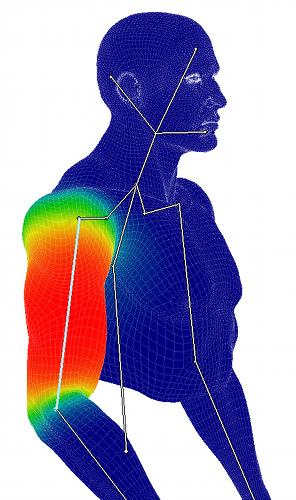
\includegraphics[width=7cm]{01_Skinning/pics/weight.png}
	\caption[Flächige Gewichtsverteilung]{ Modelldarstellung der flächigen Gewichtsverteilung auf einem Mesh. Die Farben beschreiben die Verteilung der Gewichte auf einer Skala von Blau=0, damit unabhängig, zu Rot=1, damit komplett abhängig. Entnommen von}
	\label{weights_fig1}
\end{figure}

Gewichte bezeichnen wie abhängig ein Punkt auf dem Gittergraphen bei einer Transformation von einem Knochen ist. Sie sind die Lösung um bei verformbaren Material abzuschätzen inwiefern sich jeder Punkt auf der Haut beeinflussen lässt. Dieses Gewicht $wi$ in Relation zu Knochen $i$, ist $0<=wi<=1$. Wobei 0 komplett unabhängig von dem Knochen und 1 komplett von dem Knochen abhängig ist. So wäre zum Beispiel ein Punkt auf dem Oberarm des Knochen diesem komplett mit einer 1 zugehörig, ein Punkt an der Hüfte hätte ein Gewicht von 0 am Oberarm und wäre damit komplett unabhängig von diesem. Gewichte von Punkten am Ellbogengelenk hätten variierende Werte zwischen 0 und 1. 

Nun könnten wir für jeden Vertex eine Liste erstellen mit allen seinen Gewichten in Bezug auf jedem Knochen, um zusammengefasst darzustellen wie ein Punkt sich durch das Skelett bewegen lässt. In der Summe entsprechen alle seine Gewichte immer 1, ergo $\sum_{i=1}^{N}wi=1$.

Um Gewichte zuzuordnen können verschiedene Verfahren angewandt werden, unter anderem Distanz basierte Algorithmen oder durch Lösung eines "least squares problems" (quelle). Oft ist es jedoch am effektivsten wenn durch Künstler auf Grundlage anatomischer Kenntnisse den Gittergraphen selber nach Gewichten einfärbt (quelle).